\chapter{Implementación del sistema IoT}\label{cap: }

\addcontentsline{toc}{section}{Introducción}
        \textbf{\Large Introducción}\newline
        ...\\

\section{Microcontrolador [Puede ser que halla que cambiar a ESP 12F]} \label{sec: microcontrolador}

    Un microcontrolador (abreviado: MCU) es un circuito integrado programable, capaz de ejecutar las órdenes grabadas en su memoria. Está compuesto de varios bloques funcionales, los cuales cumplen una tarea específica. Un microcontrolador incluye en su interior las tres principales unidades funcionales de una computadora: unidad central de procesamiento, memoria y periféricos de entrada/salida.\\

    El microcontrolador ESP-12F (Figura \ref{imag:esp-12F}), basado en ESP8266, posee dentro de sus características la posibilidad del empleo de la wifi como medio de comunicación.\\

    \begin{figure}[h]
        \centering
        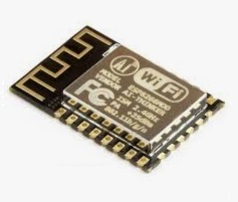
\includegraphics[width=6cm, height=6cm]{imagenes/esp-12F.jpeg}
        \caption{ESP-12F}
        \label{imag:esp-12F}
    \end{figure}

    [...]

    \vspace{4cm}

    Dentro de la familia de los ESP se encuentra el NodeMCU. Este microcontrolador (Imagen \ref{imag:nodemcu}) será el encargado de recibir los datos de los sensores y organizarlos en función de su continua transmisión hacia el concentrador.\\

    \begin{figure}[h]
        \centering
        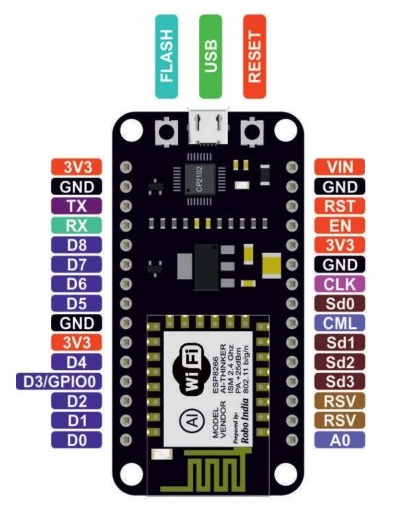
\includegraphics[width=5.5cm, height=6cm]{imagenes/nodemcu0.jpg}
        \caption{NodeMcu Vendor}
        \label{imag:nodemcu}
    \end{figure}
    
    
    NodeMCU es una pequeña placa Wifi compatible con Arduino, lista para usar en cualquier proyecto IoT. Está montada alrededor del microcontrolador ESP8266 y expone todos sus pines en los laterales. Además, ofrece más ventajas como la incorporación de un regulador de tensión integrado, así como un puerto USB de programación. Se puede programar con LUA o mediante el IDE de Arduino.\\

    Dispone de una extensa comunidad y documentación que permitirá conectar el proyecto mediante conexión Wifi.

    \textbf{Características}
    \begin{itemize}
        \item Procesador: ESP8266 a 80MHz (3.3V) (ESP-12E).
        \item 4MB de memoria FLASH (32 MBit).
        \item WiFi 802.11 b/g/n.
        \item Regulador 3.3V integrado (500mA).
        \item Conversor USB-Serial CH340G.
        \item Función Auto-reset.
        \item 9 pines GPIO con I2C y SPI.
        \item 1 entrada analógica (1.0V max).
        \item 4 agujeros de montaje (3mm).
        \item Entrada alimentación externa VIN (20V max).
    \end{itemize}

\section{Sensores} \label{sec: sensores}

    La secuencia de sensores pertenecientes al sistema es selecta, puesto que se tomaron los sensores teniendo en cuenta varios factores:

    \begin{itemize}
        \item Variable a medir
        \item Rango de operación
        \item Precisión
        \item Voltaje de alimentación
        \item Corriente de alimentación
        \item Precio
    \end{itemize}

    \vspace{3cm}

En la siguiente tabla se relacionan los mismos.

\begin{table}[h]
    \begin{tabular}{|c|c|c|cccc|}
    \hline
    \rowcolor[HTML]{9698ED} 
    \cellcolor[HTML]{9698ED}                      & \cellcolor[HTML]{9698ED}                                        & \cellcolor[HTML]{9698ED}                         & \multicolumn{4}{c|}{\cellcolor[HTML]{9698ED}Características}                                                                                                                                                                                                                          \\ \cline{4-7} 
    \rowcolor[HTML]{9698ED} 
    \multirow{-2}{*}{\cellcolor[HTML]{9698ED}No.} & \multirow{-2}{*}{\cellcolor[HTML]{9698ED}Variable}              & \multirow{-2}{*}{\cellcolor[HTML]{9698ED}Nombre} & \multicolumn{1}{c|}{\cellcolor[HTML]{9698ED}Rango}                                           & \multicolumn{1}{c|}{\cellcolor[HTML]{9698ED}Precisión} & \multicolumn{1}{c|}{\cellcolor[HTML]{9698ED}\begin{tabular}[c]{@{}c@{}}Voltaje\\ alimentación\end{tabular}} & Corriente       \\ \hline
    1                                             & \begin{tabular}[c]{@{}c@{}}Temperatura y\\ Humedad\end{tabular} & DHT22                                            & \multicolumn{1}{c|}{\begin{tabular}[c]{@{}c@{}}De - 40 a 80°C y\\ De 0 a 100RH\end{tabular}} & \multicolumn{1}{c|}{5\%}                               & \multicolumn{1}{c|}{De 3v a 6v}                                                                             & 2.5mA           \\ \hline
    2                                             & CO2                                                             & MH-Z19C                                          & \multicolumn{1}{c|}{\begin{tabular}[c]{@{}c@{}}De 400ppm a\\ 5000ppm\end{tabular}}           & \multicolumn{1}{c|}{5\%}                               & \multicolumn{1}{c|}{5v}                                                                                     & \textless{}40mA \\ \hline
    3                                             & Vibración                                                       & M0168                                            & \multicolumn{1}{c|}{\begin{tabular}[c]{@{}c@{}}Salida analógica\\ (0-1024)\end{tabular}}     & \multicolumn{1}{c|}{2\%}                               & \multicolumn{1}{c|}{De 3.3v a 5v}                                                                           & \textless{}10mA \\ \hline
    4                                             & Polución                                                        & SDS011                                           & \multicolumn{1}{c|}{\begin{tabular}[c]{@{}c@{}}De 0.0 a\\ 999.9ugm3\end{tabular}}            & \multicolumn{1}{c|}{10\%}                              & \multicolumn{1}{c|}{5v}                                                                                     & 100mA           \\ \hline
                                                  &                                                                 & LDR                                              & \multicolumn{1}{c|}{}                                                                        & \multicolumn{1}{c|}{}                                  & \multicolumn{1}{c|}{5v}                                                                                     & 10mA            \\ \cline{3-7} 
    \multirow{-2}{*}{5}                           & \multirow{-2}{*}{Luz}                                           & BH1750                                           & \multicolumn{1}{c|}{De 1 a 65535 lx}                                                         & \multicolumn{1}{c|}{20\%}                              & \multicolumn{1}{c|}{De 2.4v a 3.6v}                                                                         & 0.12mA          \\ \hline
    \end{tabular}
    \caption{Relación sensores}
    \subcaption*{Fuente: Elaboración propia}
    \label{tab:relacion_sensores}
\end{table}

\subsection{Descripción sensores} \label{subsec: descripcion_sensores}

\addcontentsline{toc}{subsection}{\hspace{1.3cm}2.2.1.1\hspace{5mm}Sensor DHT22}
        \textbf{\large 2.2.1.1\hspace{5mm}Sensor DHT22}

  \begin{figure}[h]
      \centering
      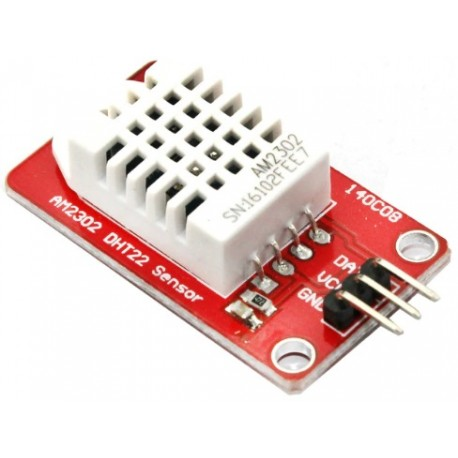
\includegraphics[width=5cm, height=5cm]{imagenes/dht22.jpg}
      \caption{Sensor DHT22}
      \subcaption*{Fuente: Datasheet fabricante}
      \label{imag:dht22}
   \end{figure}
   
El DHT22 (AM2302) es un sensor digital de temperatura y humedad relativa de buen rendimiento y de bajo costo. Integra un sensor capacitivo de humedad y un termistor para medir el aire circundante, y muestra los datos mediante una señal digital en el pin de datos (no posee salida analógica).\\

\begin{figure}[h]
    \centering
    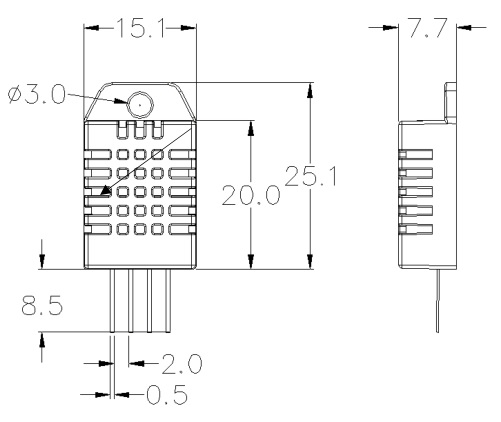
\includegraphics[width=8cm, height=6cm]{imagenes/dht22 dimensiones.jpg}
    \caption{Dimensiones sensor DHT22}
    \label{imag:dimensiones_dht22}
\end{figure}

\vspace{1cm}

\addcontentsline{toc}{subsection}{\hspace{1.3cm}2.2.1.2\hspace{5mm}Sensor MZ-Z19C}
        \textbf{\large 2.2.1.2\hspace{5mm}Sensor MZ-Z19C}

\begin{figure}[h]
      \centering
      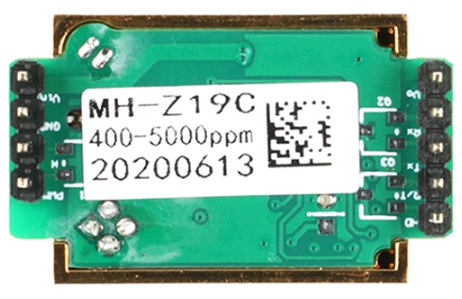
\includegraphics[width=5cm, height=3cm]{imagenes/mh-z19c.png}
      \caption{Sensor MH-Z19C}
      \label{imag:mh-z19c}
   \end{figure}

El sensor de gas de dióxido de carbono MH-Z19C es un pequeño sensor inteligente de uso general que utiliza el principio del infrarrojo no disperso (NDIR) para detectar la presencia de CO2 en el aire.\\

\textbf{Otros datos}
\begin{itemize}
    \item Señal de salida: UART(TTL)
    \item Tiempo de precalentamiento: 60 segundos
    \item Temperatura de operación: De -10 a 50°C
    \item Humedad de operación: De 0 - 95 por ciento RH
    \item Dimensiones: aprox. 39 x 20 x 9 mm
    \item Tipo de conector: JST ZH de 7 pines
\end{itemize}

\vspace{2cm}

\addcontentsline{toc}{subsection}{\hspace{1.3cm}2.2.1.3\hspace{5mm}Sensor M0168}
        \textbf{\large 2.2.1.3\hspace{5mm}Sensor M0168}

\begin{figure}[h]
      \centering
      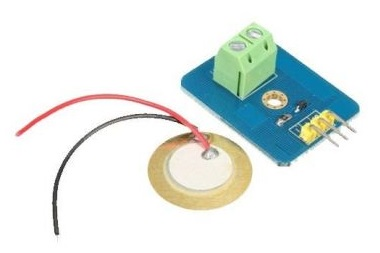
\includegraphics[width=6.5cm, height=5cm]{imagenes/sensor-piezoelectrico.jpg}
      \caption{Sensor piezoeléctrico M0168}
      \label{imag:M0168}
   \end{figure}

En este sensor piezoeléctrico cuando el choque de la cerámica con la lámina metálica genera una señal eléctrica, esta señal analógica es la recibida por los pines analógicos de microcontroladores.\\

\textbf{Especificaciones Técnicas}

\begin{itemize}
    \item Voltaje de trabajo: 3.3V o 5V
    \item Corriente de trabajo: 1mA
    \item Rango de temperatura de funcionamiento: -10 ~ +70
    \item Interfaz Tipo: salida analógica
    \item Tamaño del artículo: 30mm x 23mm
\end{itemize}

\vspace*{1cm}

\addcontentsline{toc}{subsection}{\hspace{1.3cm}2.2.1.4\hspace{5mm}Sensor SDS011}
        \textbf{\large 2.2.1.4\hspace{5mm}Sensor SDS011}

\begin{figure}[h]
      \centering
      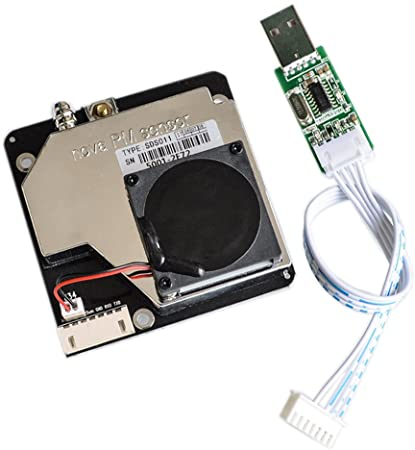
\includegraphics[width=4.5cm, height=4.5cm]{imagenes/Sensor SDS011.jpg}
      \caption{Sensor SDS011}
      \label{imag:SDS011}
   \end{figure}

Se basa en el principio de dispersión láser: se puede inducir la dispersión de la luz cuando las partículas atraviesan el área de detección. La luz dispersa se transforma en señales eléctricas, después estas señales serán amplificadas y procesadas. El número y el diámetro de las partículas se pueden obtener mediante análisis porque la forma de onda tiene ciertas relaciones con el diámetro de las partículas.\\

\vspace{2cm}

\textbf{Otros datos}

\begin{itemize}
    \item Corriente del sueño: 2mA
    \item Frecuencia de muestreo serie: 1 segundo
    \item Resolución diámetro de partículas: <= 0.3um
    \item Rango de temperatura: -20 a 50°C
    \item Tamaño físico: 71mm x 70mm x 23mm 
\end{itemize}

\vspace{1cm}

\addcontentsline{toc}{subsection}{\hspace{1.3cm}2.2.1.5\hspace{5mm}Sensor LDR}
        \textbf{\large 2.2.1.5\hspace{5mm}Sensor LDR}\newline

\begin{figure}[h]
      \centering
      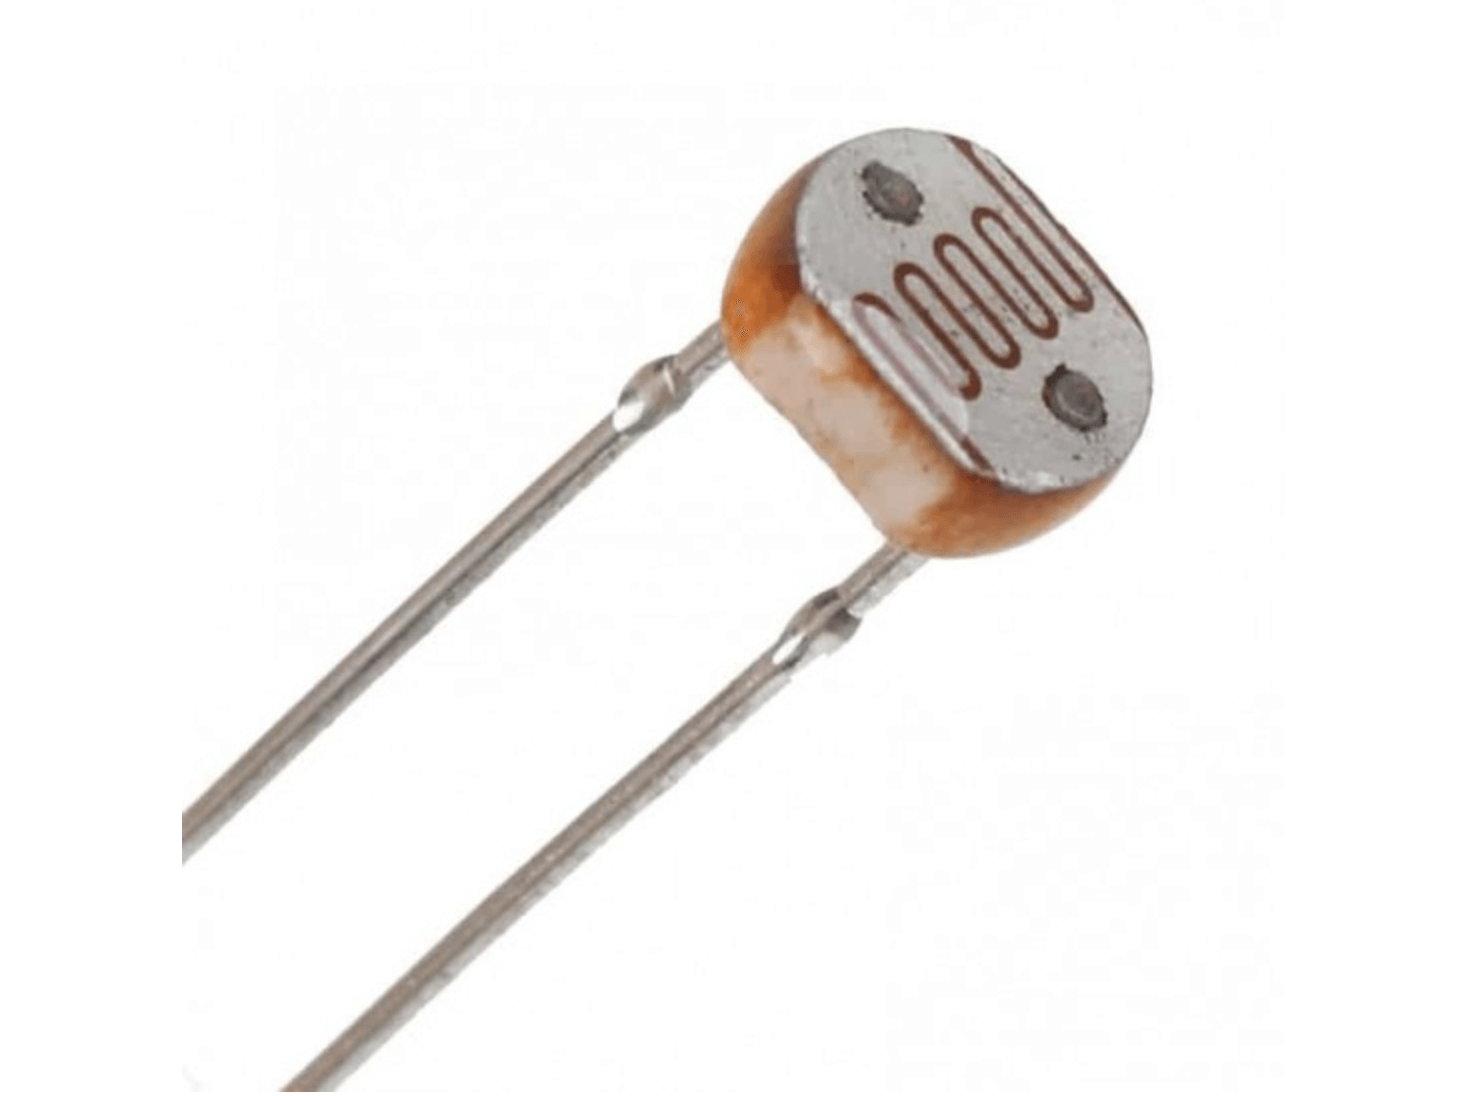
\includegraphics[width=5.5cm, height=4cm]{imagenes/sensor LDR.png}
      \caption{Sensor LDR}
      \label{imag:LDR}
   \end{figure}

Una fotorresistencia es un componente electrónico cuya resistencia disminuye con el aumento de la intensidad de la luz incidente. Puede también ser llamado fotorresistor, fotoconductor, célula fotoeléctrica o resistor dependiente de la luz, cuyas siglas, LDR, se originan de su nombre en inglés light-dependent resistor.\\

\begin{figure}[h]
    \centering
    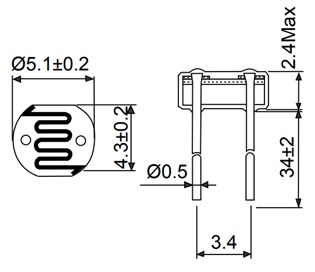
\includegraphics[width=4.5cm, height=4cm]{imagenes/ldr.jpg}
    \caption{Sensor LDR}
    \subcaption*{Fuente: Datasheet fabricante}
    \label{imag:dimensiones LDR}
 \end{figure}

\vspace{1cm}

\addcontentsline{toc}{subsection}{\hspace{1.3cm}2.2.1.6\hspace{5mm}Sensor BH1750}
        \textbf{\large 2.2.1.6\hspace{5mm}Sensor BH1750}\newline

\begin{figure}[h]
      \centering
      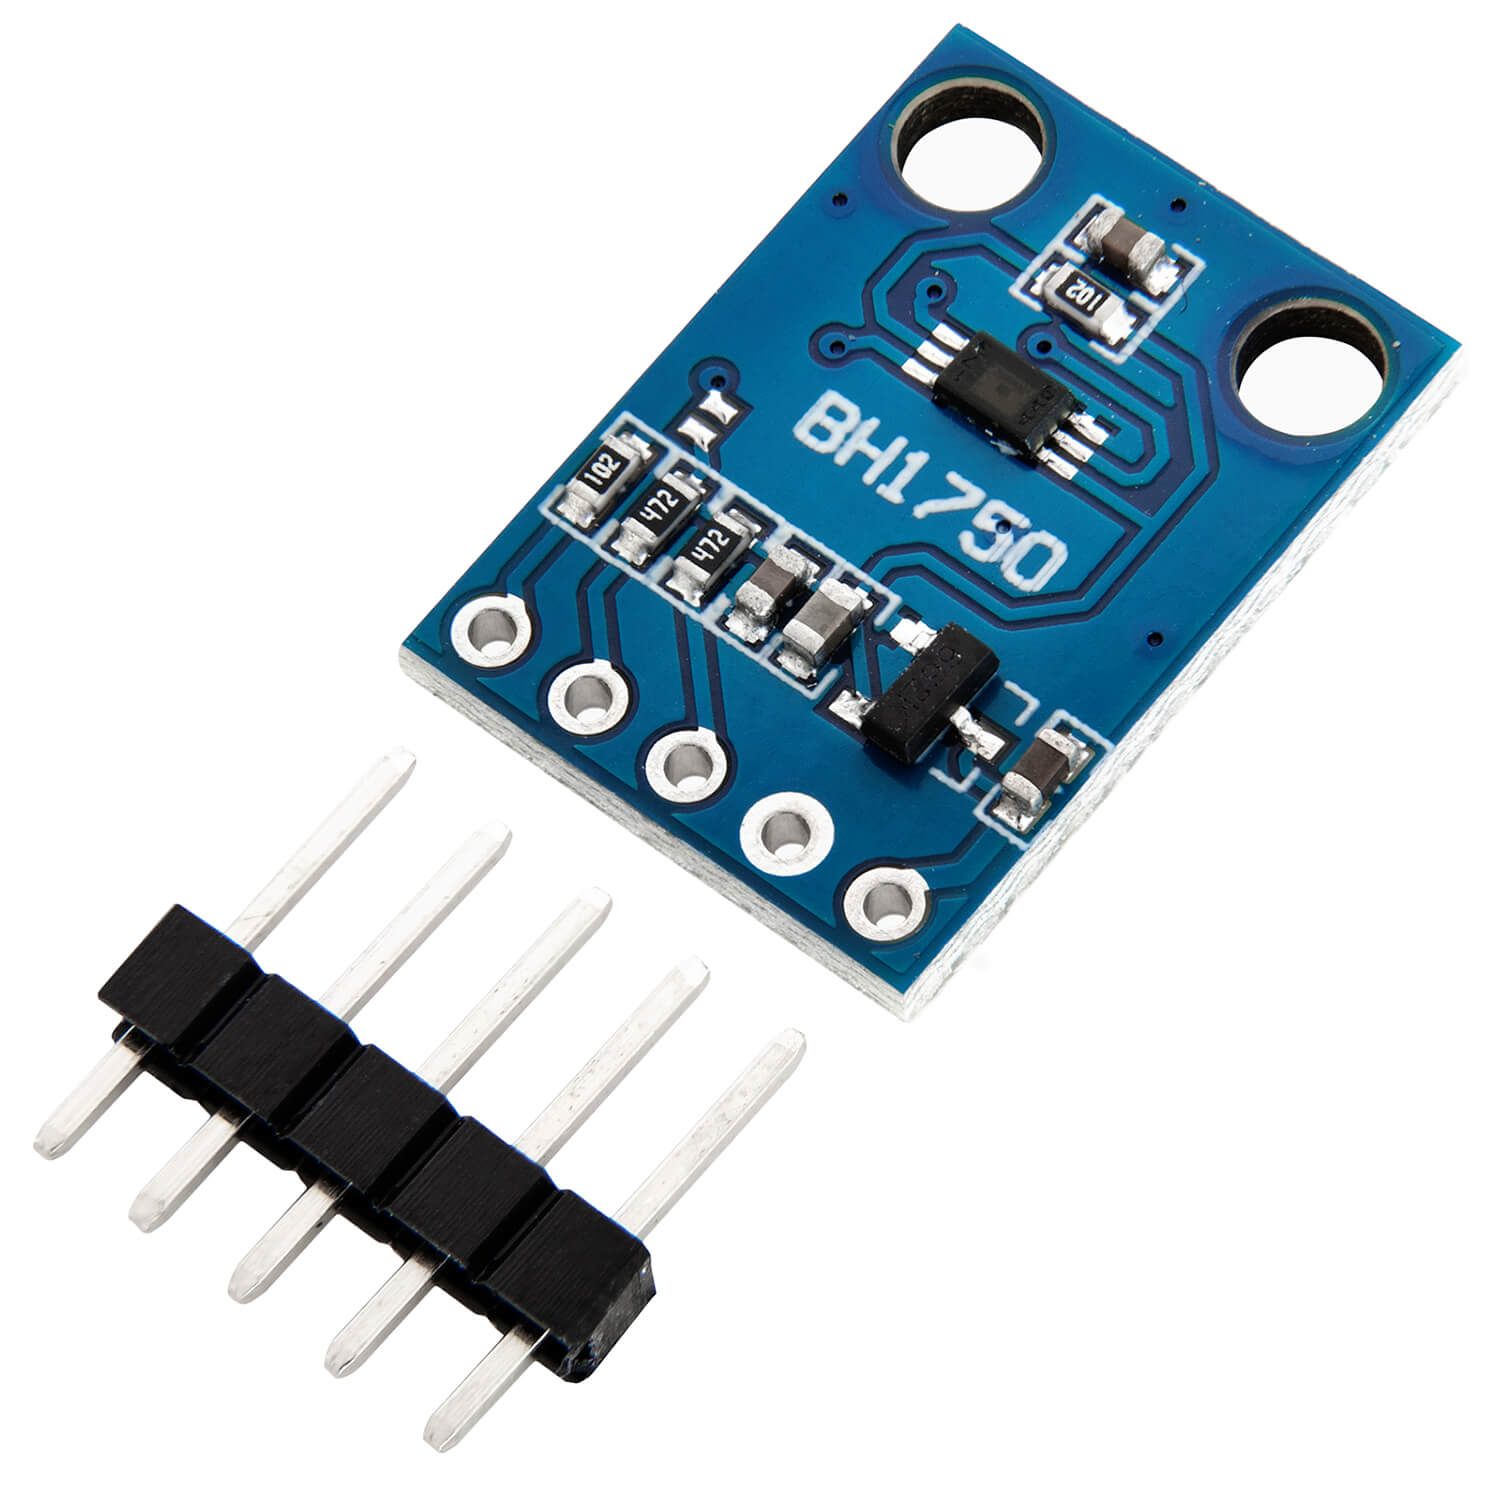
\includegraphics[width=5cm, height=4cm]{imagenes/Sensor BH1750.jpg}
      \caption{Sensor BH1750}
      \label{imag:BH1750}
   \end{figure}

El Módulo BH1750 es un sensor de iluminación digital para medición de flujo luminoso (iluminancia) de la empresa Rohm Semiconductor. Componente que posee dentro de su arquitectura interna, un conversor análogo digital (ADC) de 16 bits con una salida digital de formato I2C, que facilita la integración con microcontroladores o sistemas embebidos diversos. Este módulo entrega la intensidad luminosa directamente en unidades de Lux que es equivalente a Lumen/m2.\\

\textbf{Otros datos}

\begin{itemize}
    \item Interfaz Digital: I2C
    \item Frecuencia máxima de transmisión: 400kHZ
    \item Temperatura de operación: Desde -40°C hasta 85°C
\end{itemize}

\vspace{2cm}

Para su correcto funcionamiento, este sensor debe ir acompañado de una serie de componentes electrónicos para su acondicionamiento.
En la figura \ref{imag:acondicionamiento_BH1750} se puede observar el acondicionamiento brindado por el fabricante.

\begin{figure}[h]
    \centering
    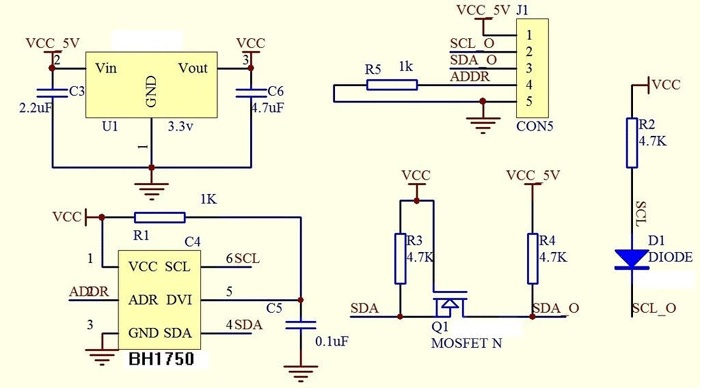
\includegraphics[width=11cm, height=7cm]{imagenes/acondicionamientos sensor BH1750.jpg}
    \caption{Acondicionamiento sensor BH1750}
    \subcaption*{Fuente: Datasheet fabricante}
    \label{imag:acondicionamiento_BH1750}
\end{figure}

\addcontentsline{toc}{section}{Conclusiones}
        \textbf{\Large Conclusiones}\newline
